\documentclass[../mciAusarbeitung.tex]{subfiles}

\usepackage[utf8]{inputenc}
\usepackage[T1]{fontenc}
\usepackage{lmodern}
\usepackage[german]{babel}
\usepackage[fixlanguage]{babelbib}
\selectbiblanguage{german}
\usepackage{amssymb}
\usepackage{graphicx}
\usepackage{url}
\usepackage{float}

\title{Fachpraktikum MCI (01513) - WS 2021/22}
\author{Gruppe 2\\
	Sabine Hopf}
\date{\today}

\begin{document}
	Es wurden Generatoren aus drei unterschiedlichen Kategorien implementiert, die nachfolgend beschrieben werden. Außerdem wird die Varianz der Generatoren und deren Kooperationsmöglichkeiten vorgestellt.\\
	\subsubsection{L-System}
		L-Systeme oder Lindenmayer-Systeme sind Systeme, die sich auf künstlerischer Ebene eignen, realitätsnahe Pflanzenmodellierungen oder andere Fraktale zu generieren. \\
		Das wesentliche Prinzip besteht darin, nach und nach einzelne Symbole mit entsprechenden Produktionsregeln durch andere Symbole zu ersetzen und dies bis zu einer Tiefe n rekursiv auszuführen. Durch eine sogenannte Turtle-Grafik werden dann die Symbole in entsprechende Linien oder Winkel transformiert.
		Dabei besteht das L-System aus einem Alphabet V aus Terminal- und Nichtterminalsymbolen, einem Startwort $\omega  $ aus dem Alphabet V und Produktionsregeln P, die festlegen, welche Nichtterminalsymbole durch welche Symbole oder Abfolge von Symbolen ersetzt werden sollen.\\
		Als Beispiel:\\
		\\
		n = 0\\
		$ \omega $ = F\\
		P = F->F[-F]\\
		Diese würde bei n = 1 bedeuten:\\
		F[-F]\\
		bei n = 2:\\
		F[-F][-F[-F]] usw.\\
		\\
		Die Visualisierung dieser Symbole wird nun so realisiert, dass man sich bildlich eine Schildkröte (daher Turtle-Grafik) vorstellt, die mit einem Stift über den Bildschirm läuft und an den entsprechenden Symbolen z. B. Linien zeichnet (hier z. B. beim 'F') und bei einem anderen Symbol (hier z. B. bei '-') die Richtung in einem bestimmten Winkel ändert. Durch einen LIFO-Speicher (Last In First Out) wird bei dem Symbol '[' der aktuelle Zustand, also die Position und Richtung der Schildkröte (bzw. das aktuelle Koordinatensystem) auf dem  Stack gespeichert und bei dem Symbol ']' der oberste Zustand vom Stack entfernt und zum aktuellen Zustand gemacht.\\
		L-Systeme können nicht nur für Pflanzenmodellierungen genutzt werden, sondern z. B. auch für Kochsche Schneeflocken und Drachenkurven.\\
		\paragraph{Beschreibung der Implementierung}$~$\\
		Die Implementierung erfolgte inspiriert von 'The nature of code' \cite{shiffman2012nature} wie oben beschrieben.
		Es wurden mit Hilfe der Produktregeln von 'The algorithmic beauty of plants'  \cite{prusinkiewicz2012algorithmic} S. 25, verschiedene Regeln für unterschiedliche Bäume implementiert.\\
		Die Regeln werden nach Auswahl des entsprechenden Baumes aus einem Rules-Array geladen und ausgeführt.\\
		Die Bäume sind parametrisierbar durch ihren Startpunkt in x und y Richtung, die Farbe der Zweige und der Anfangsrotation des Baumes. Außerdem kann die Anzahl der Bäume gewählt werden, im Bereich von 1 bis 10.\\
		Die Winkelgröße und die Länge der Zweige werden gegebenenfalls durch die Parameter der anderen Generatoren beeinflusst und können deshalb nicht individuell eingestellt werden. Außerdem entarten die Bäume, wenn der Zufallsparameter kleiner als 0,5 ist. Dieser Wert wurde willkürlich gewählt, um noch mehr Variationen zu erzeugen. Auch die Startpunkte und die Alphawerte der Bäume > 1 werden durch den Zufallsparameter beeinflusst. Gleichzeitig berechnet der Algorithmus noch einen Punkt, der im ersten Baum liegt, der von anderen Generatoren als Kooperation genutzt werden kann.\\
		Der Algorithmus benutzt seinerseits den Kooperationspunkt, um zu entscheiden, zu welcher Richtung manche Bäume gezeichnet werden. Ist die x-Koordinate des Kooperationspunktes größer als die halbe Weite des Zeichenfensters, wird der Baum zur jeweils anderen Seite als der normalen Seite ausgerichtet, außerdem variiert der Alpha-Wert der Farbe.\\
		
		\paragraph{Beispiele}$~$\\
		Unten wurde das Beispiel aus der Aufgabenstellung nachgebaut. Daneben wurde nur der x-Wert der Startposition über die Mitte des Bildes verschoben. Man kann erkennen, wie sich die Richtung des Baumes verändert hat, außerdem variiert der Alpha-Wert der Farbe:\\
		Bildgenerierung links:,,Menübar/Beispiele/SHopf/L-System/TreeBeispiel''\\
		Bildgenerierung rechts:,,Menübar/Beispiele/SHopf/L-System/TreeBeispielRichtung''\\
		\begin{figure}[H]
			\begin{minipage}[t]{0.45\linewidth} 
				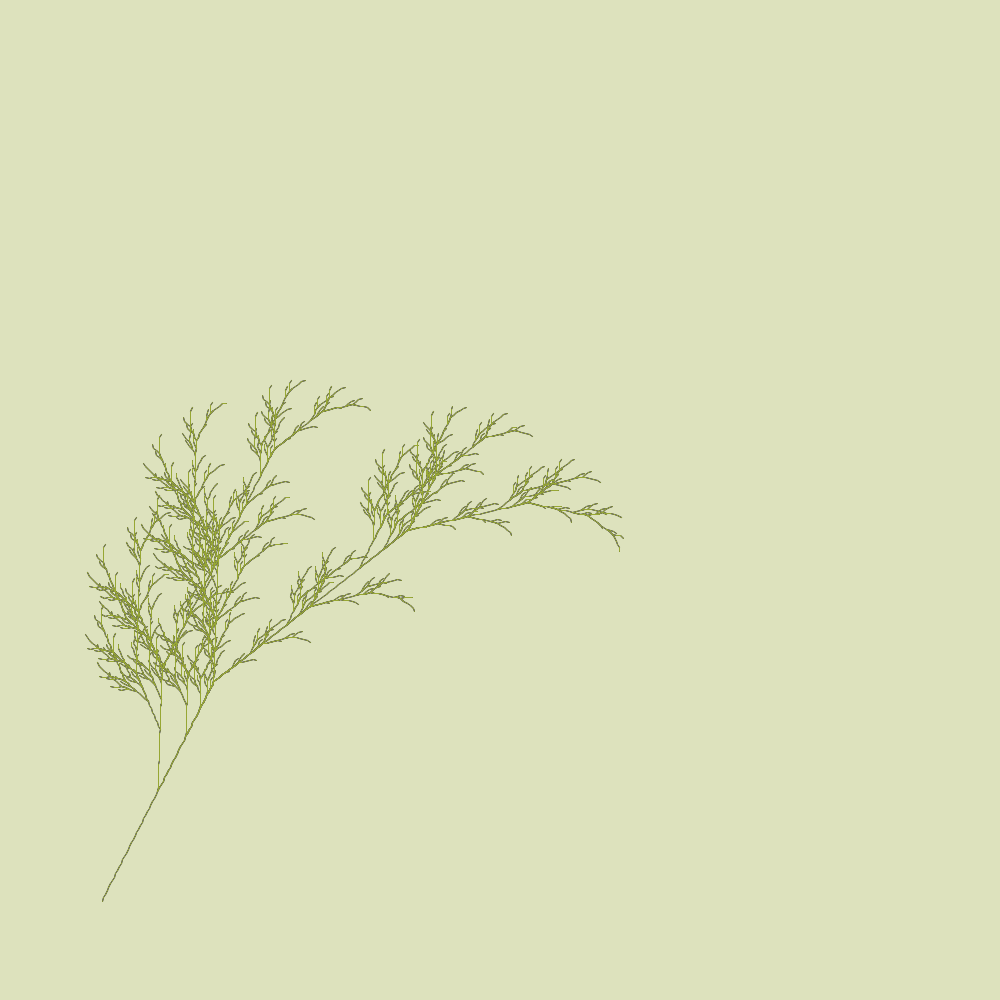
\includegraphics[width=\linewidth]{img/treeBeispiel.png}
				\caption[TreeBeispiel]{Beispiel aus Aufgabenstellung (eigene Darstellung)}
			\end{minipage}
			\hfill
			\begin{minipage}[t]{0.45\linewidth} 
				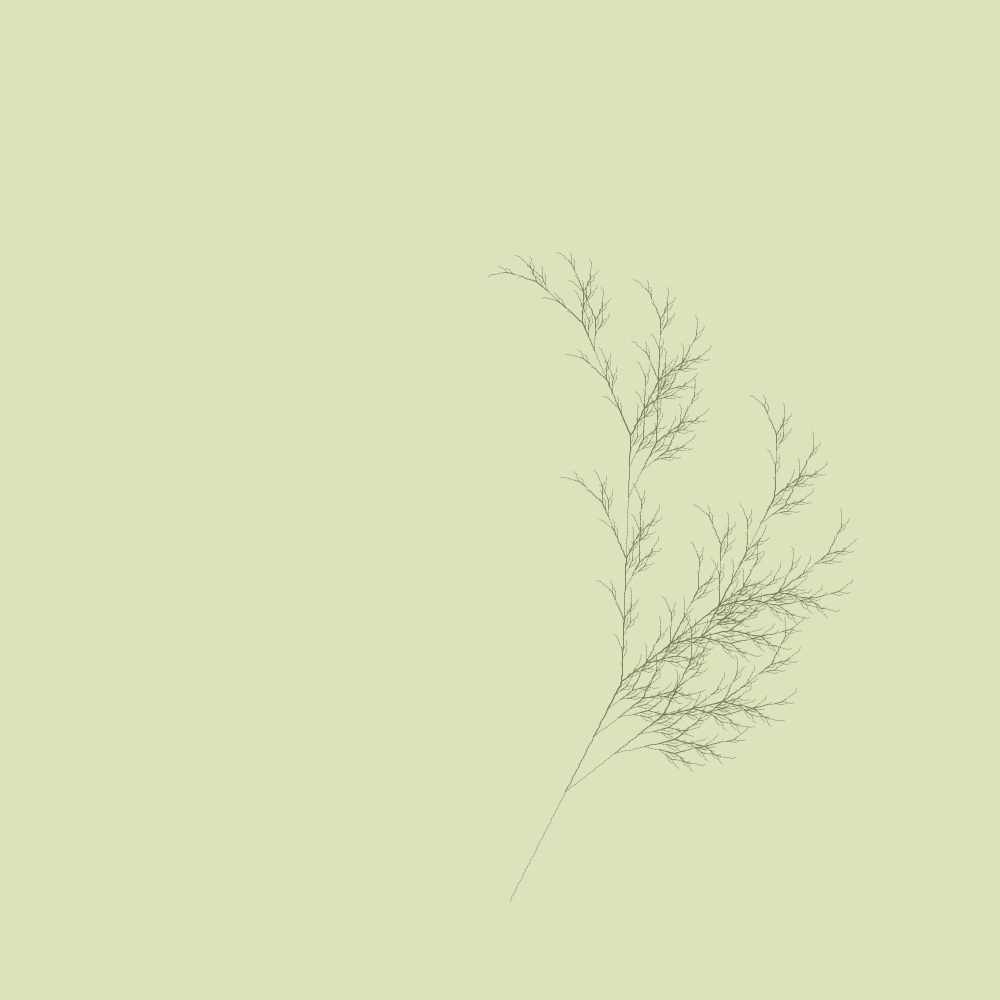
\includegraphics[width=\linewidth]{img/treeRichtung.png}
				\caption[TreeBeispielRichtung]{Beispiel aus Aufgabenstellung mit verschobenem x-Wert (eigene Darstellung)}
			\end{minipage}
		\end{figure}
		\noindent Unten wurde die Anfangsrotation so weit gestellt, dass auch Abbildungen auf dem Kopf möglich sind:\\
		Bildgenerierung:,,Menübar/Beispiele/SHopf/L-System/TreeKopf''\\
		\begin{figure}[H]
			\centering
			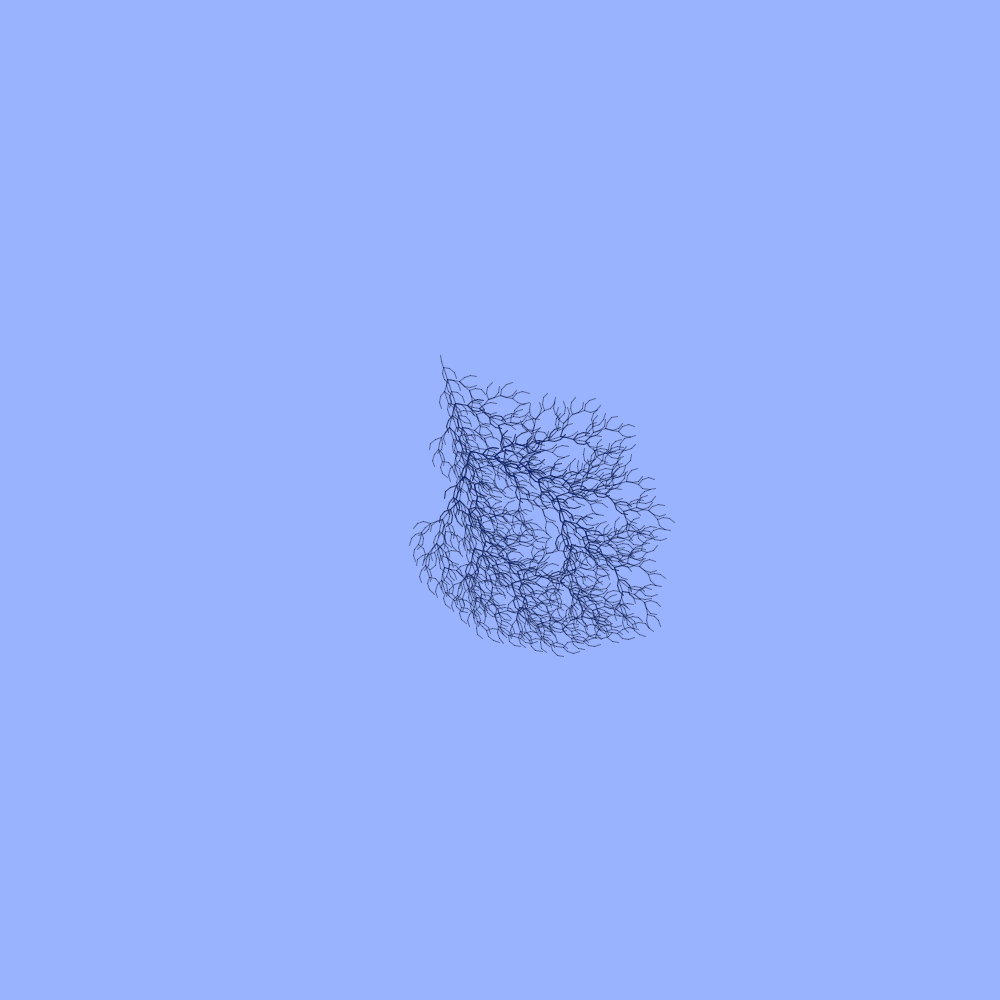
\includegraphics[width=0.5\linewidth]{img/treeKopf.png}
			\caption[TreeKopf]{Baum auf dem Kopf (eigene Darstellung)}
		\end{figure}
		\noindent Unten wurde die Anzahl der Bäume auf 10 gestellt. Hier kann man noch mal alle Variationen erkennen, wie die Bäume die Richtung ändern und der Alphawert variiert:\\
		Bildgenerierung:,,Menübar/Beispiele/SHopf/L-System/TreeRichtung''\\
		\begin{figure}[H]
			\centering
			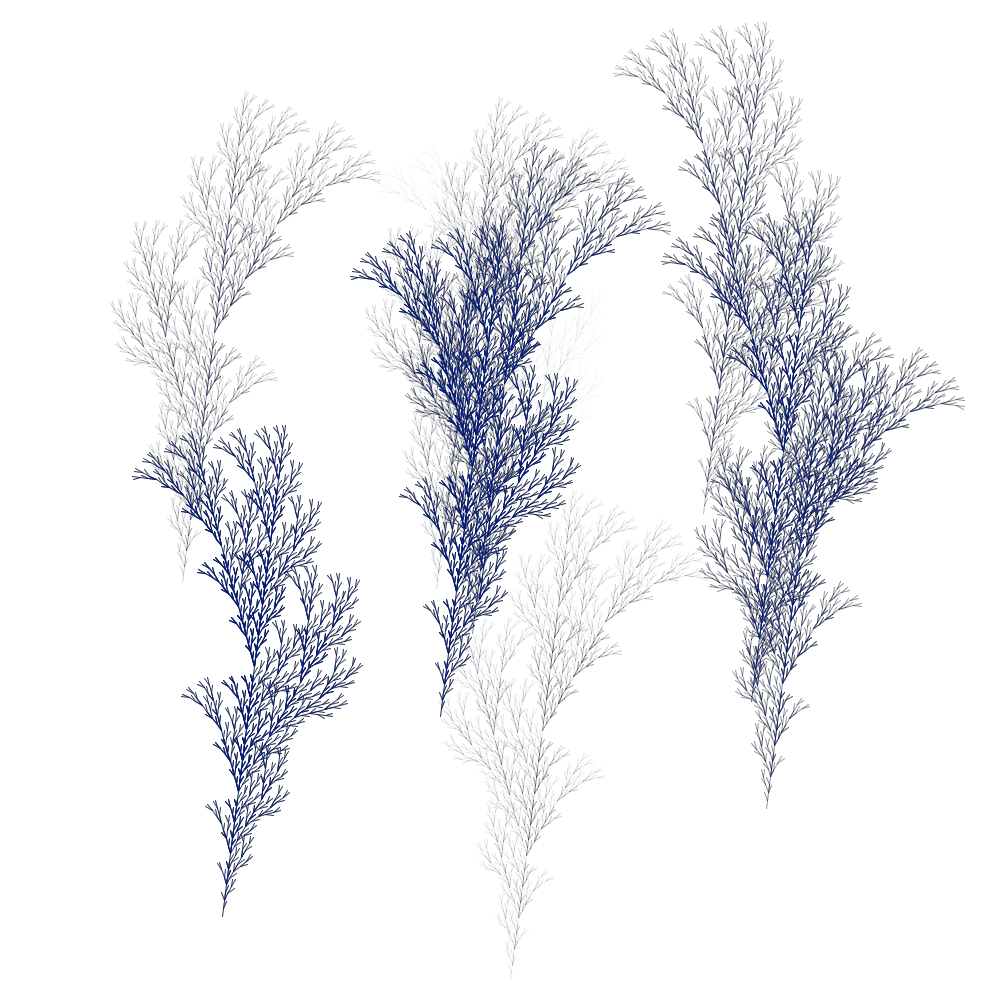
\includegraphics[width=0.5\linewidth]{img/tree10Richtung.png}
			\caption[TreeRichtung]{10 Bäume Variation (eigene Darstellung)}
		\end{figure}
		\noindent Unten wurden nochmal alle Bäume kombiniert. Man kann sehen, dass zu den anderen Variationen noch hinzu kommt, dass Bäume entarten und sich die Größe der Bäume unterscheidet:\\
		Bildgenerierung:,,Menübar/Beispiele/SHopf/L-System/TreeKombi''\\
		\begin{figure}[H]
			\centering
			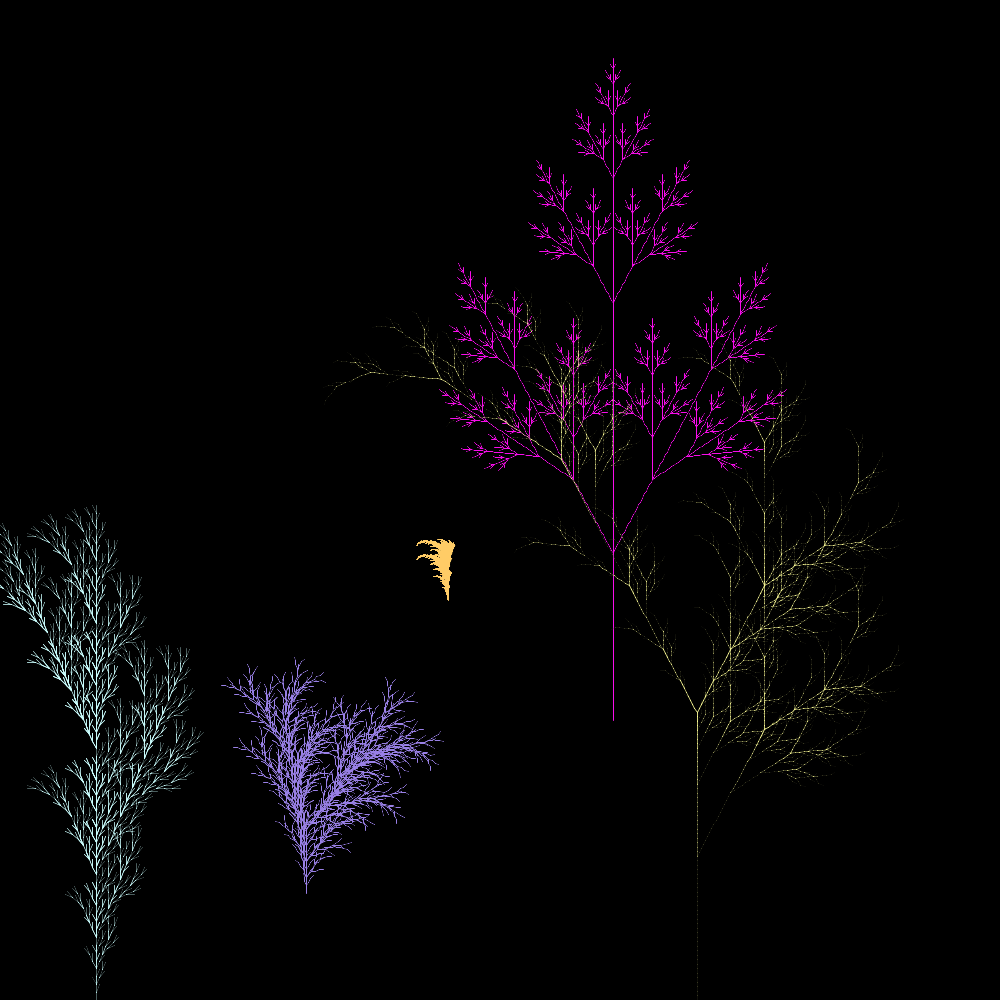
\includegraphics[width=\linewidth]{img/treeKombi.png}
			\caption[TreeKombi]{Verschiedene Bäume Variationen (eigene Darstellung)}
		\end{figure}
		
				
		
		\paragraph{Stärken und Schwächen}$~$\\
		Die Stärken des L-Systems liegen sicherlich darin, dass mit einem relativ einfachen Algorithmus erstaunlich komplexe Gebilde erschaffen werden können. Auf der anderen Seite darf die Rekursionstiefe $ n $ speziell bei den Bäumen nicht zu hoch sein, da sonst der Speicherplatz exponentiell wächst.\\
		Der Algorithmus ist auf jeden Fall für die Einzelgenerierung geeignet, da man dort Größe und Ausrichtung des Baumes auf die Größe des Bildes und den Geschmack des Betrachters ausrichten kann. Bei der Kooperation ist dies nicht unbedingt gegeben. Der Winkel der Zweige kann so klein werden, dass nur noch ein Strich übrig bleibt. Der Baum kann auch so klein werden, dass er fast nicht mehr gesehen wird, oder so groß, dass er nicht mehr ins Bild passt. Vielleicht kann aber auch dieser Zufall gerade den Reiz des Bildes ausmachen.
	 
	 
	\subsubsection{Simulation von Schwarmverhalten}
		Synchronisiertes Gruppenverhalten in Herden oder Schwärmen, egal ob von Fischen, Vögeln oder Säugetieren sind die Vorlage für diesen Algorithmus. Dabei kann man leicht vermuten, dass es bei diesem Verhalten einen Anführer geben muss, der die anderen Gruppenmitglieder auf irgendeine Art und Weise anleitet oder führt. Es deutet aber alles darauf hin, dass die gemeinsame Bewegung ein summiertes Verhalten der einzelnen Individuen sein muss.\\
		Craig Reynolds beschreibt in seinem Artikel ,,Flocks, Herds, and Schools: A Distributed Behavioral Model'' \cite{reynolds1987flocks} einen einfachen Ansatz ein Schwarmverhalten zu simulieren. Angelehnt an ein Particle-System, bei dem eine große Ansammlung einzelner Teilchen jeweils ein eigenes Verhalten hat, hat er seine sogenannten ,,Boids'' erschaffen. Diese haben jeweils ein eigenes Verhalten, welches er auf drei Steuerungsmechanismen reduziert. Alignment, Cohesion und Separation.
		\begin{itemize}
			\item Alignment steht dabei für Ausrichtung auf den durchschnittlichen Kurs der anderen
			\item Cohesion steht dabei für Zusammenhalt bezüglich der durchschnittliche Position der anderen
			\item Separation steht dabei für Trennung, d. h. ein gewisser Abstand, bzw. Freiraum zu den anderen
		\end{itemize}
		Jeder Boid reagiert nur auf die Geschehnisse in seiner Nachbarschaft. Hier kann also ein bestimmter Radius eingestellt werden, in dem ein Boid die anderen Boids ,,sieht''. Auch dies ist dem Wahrnehmungskreis der Individuen in der Natur nachempfunden, z. B. wenn Fische im trüben Wasser schwimmen.
		\paragraph{Beschreibung der Implementierung}$~$\\
		Die Implementierung erfolgte inspiriert von 'The nature of code' \cite{shiffman2012nature} wie oben beschrieben.
		Zuerst werden die Boids erstellt. Die Anzahl der Boids sind parametrisiert und können im Bereich von 1 bis 1000 gewählt werden. Außerdem ist auch das Aussehen der Boids parametrisiert und der Benutzer hat die Auswahl zwischen Punkten, Kurven und Dreiecken. Die Boids werden zunächst zufallsmäßig auf dem Bildschirm verteilt. Dieser Zufall wird allerdings im ganzen Algorithmus, bzw. in allen Generatoren durch Pseudozufallszahlen ermittelt, die durch einen seed inititalisiert werden. Damit ist sichergestellt, dass die Bildgenerierung deterministisch bleibt.\\
		Weiterhin erhält jeder Boid eine zufällige Geschwindigkeit und eine zufällige Farbe aus dem Regenbogenspektrum. Dann berechnet jeder Boid die durchschnittliche Ausrichtung der anderen Boids in seinem Wahrnehmungskreis und lenkt dementsprechend in diese Richtung. Genauso lenkt er sich in die durchschnittliche Position mit gleichzeitiger Wahrung des Abstandes zu den anderen Boids. So entstehen immer wieder kleinere Gruppen, die das Schwarmverhalten simulisieren.\\
		Als Besonderheit in diesem Algorithmus nehmen die Boids die Farbe ihrer Nachbarn im Wahrnehmungskreis an. Wenn sie sich von der Gruppe entfernen, nehmen sie wieder ihre Originalfarbe an.\\
		Als weitere Parametrisierung kann die Wahrung des Abstandes zu anderen Boids eingestellt werden. Damit noch andere Kräfte auf den Schwarm wirken, enthält der Algorithmus noch ein Hindernis, bei dem der Benutzer die Stärke der Abwehrkraft einstellen kann. Diese bewirkt, dass die Boids dieses Hindernis meiden. Das Hindernis kann wahlweise sichtbar oder unsichtbar eingestellt werden.\\
		Dadurch, dass ein Boid nur die anderen Boids in seinem Wahrnehmungskreis berechnen muss, ist der Algortihmus etwas effektiver, als wenn er alle Boids auf der gesamten Zeichenfläche berechnen müsste. Möglich macht dies die Einbindung eines Quadtrees, bei dem die Zeichenfläche zunächst in vier Quadrate unterteilt wird. In jedem Quadrat dürfen sich höchstens vier Boids aufhalten. Werden es mehr, teilt sich das Quadrat wieder in vier Quadrate usw. Dies wird rekursiv ausgeführt. Auch der Quadtree kann wahlweise sichtbar oder unsichtbar eingestellt werden, aus künstlerischen Gründen, aber auch wenn man diesen einfach mal in Aktion sehen möchte.\\
		Die Kooperation mit anderen Generatoren erfolgt einerseits mit den pseudozufallsmäßigen Variablen, die die Startpositionen der Boids und die Anfangsgeschwindigkeit beeinflussen, da der Seed durch die Parametrisierung aller beteiligten Generatoren beeinflusst wird. Auf der anderen Seite kann der Standort des Hindernisses von anderen Generatoren beeinflusst werden, wenn diese ein Interface benutzen, in dem sie diesen Punkt berechnen.\\
		Der Algorithmus gibt seinerseits den Standort des Hindernisses als Kooperationspunkt weiter.\\
		
		\paragraph{Beispiele}$~$\\
		Unten sieht man 850 Boids in der Gestalt von Kurven mit Hindernis:\\
		Bildgenerierung:,,Menübar/Beispiele/SHopf/Schwarm/SchwarmKurven''\\
		\begin{figure}[H]
			\centering
			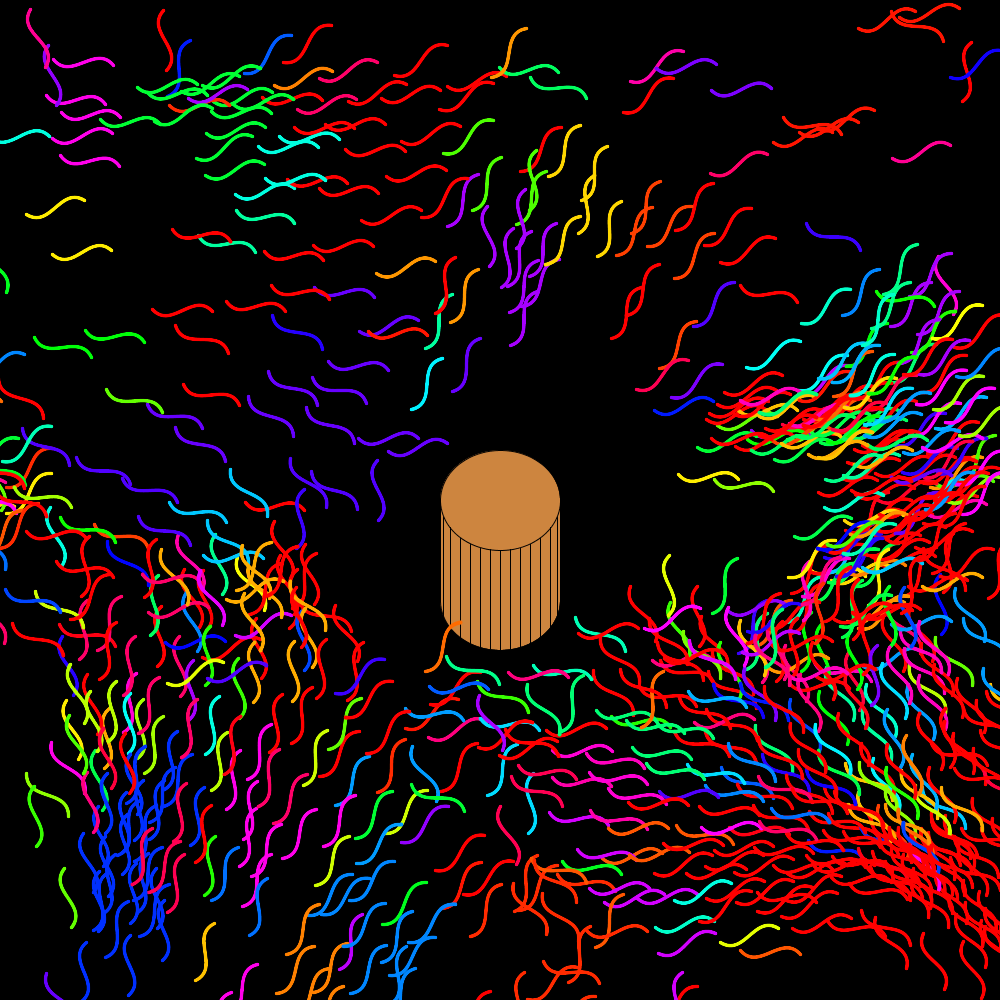
\includegraphics[width=0.5\linewidth]{img/schwarmKurven.png}
			\caption[SchwarmKurven]{Schwarm mit 850 Individuen und Hindernis (eigene Darstellung)}
		\end{figure}
		\noindent Unten wurde die Separation der Boids auf 5 gestellt. Damit wurde eine Verklumpung der Schwarmgruppen erreicht. Man kann gut erkennen, dass zwar das Hindernis nicht sichtbar geschaltet ist, dieses aber trotzdem den Abwehrmechanismus ausgelöst hat. Hier kann man weiterhin sichtbar machen, wie der Quadtree arbeitet. Es gibt viele kleine Quadrate an den Verklumpungen und nur große Quadrate, wo sich keine Boids aufhalten.\\
		Bildgenerierung:,,Menübar/Beispiele/SHopf/Schwarm/SchwarmQuad''\\
		\begin{figure}[H]
			\centering
			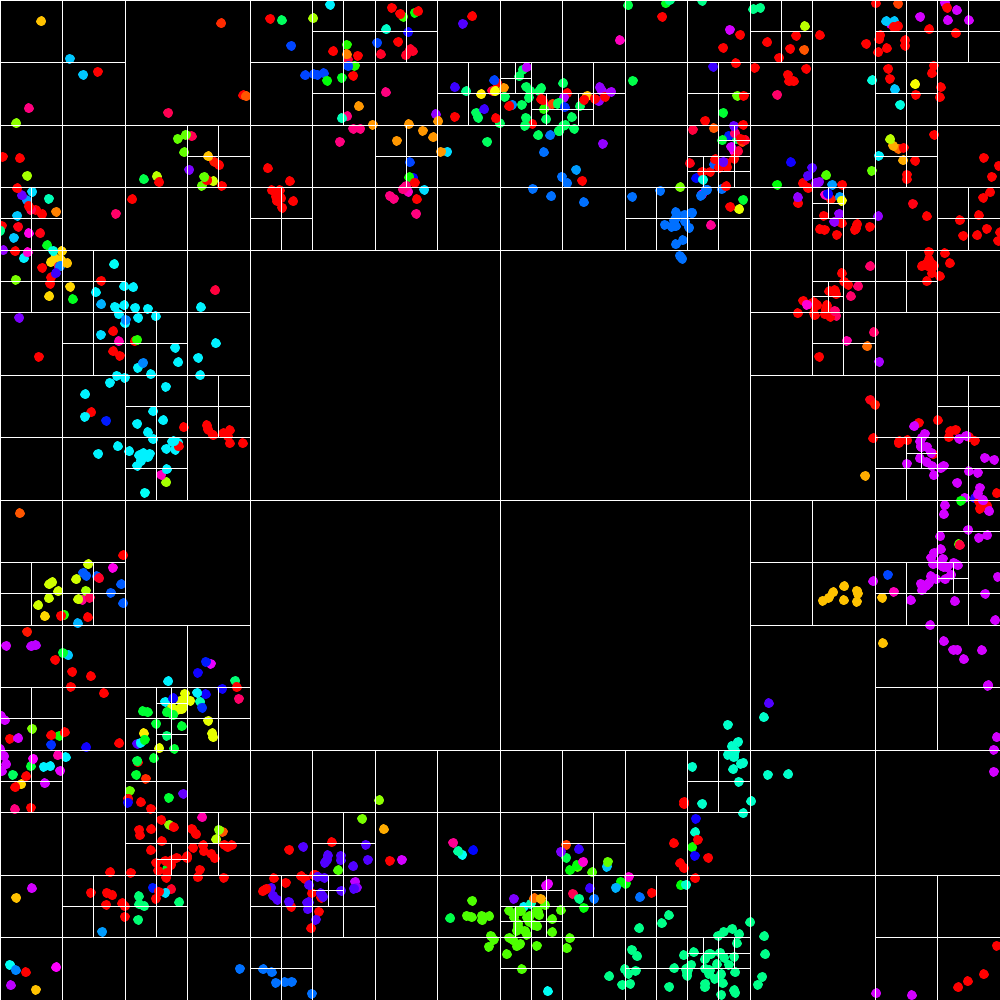
\includegraphics[width=0.5\linewidth]{img/schwarmQuad.png}
			\caption[SchwarmQuad]{Schwarm mit Separation 5 und Quadtree (eigene Darstellung)}
		\end{figure}
		\noindent Unten wurde der Verlauf der Kurven-Boids ausgeschaltet. Dadurch, dass diesmal die Separation der Boids auf 100 geschaltet wurde, versucht jedes Individuum möglichst allein für sich zu ,,schwimmen''. Dadurch ergeben sich schöne Verläufe.\\
		Bildgenerierung:,,Menübar/Beispiele/SHopf/Schwarm/SchwarmKunst''\\
		\begin{figure}[H]
			\centering
			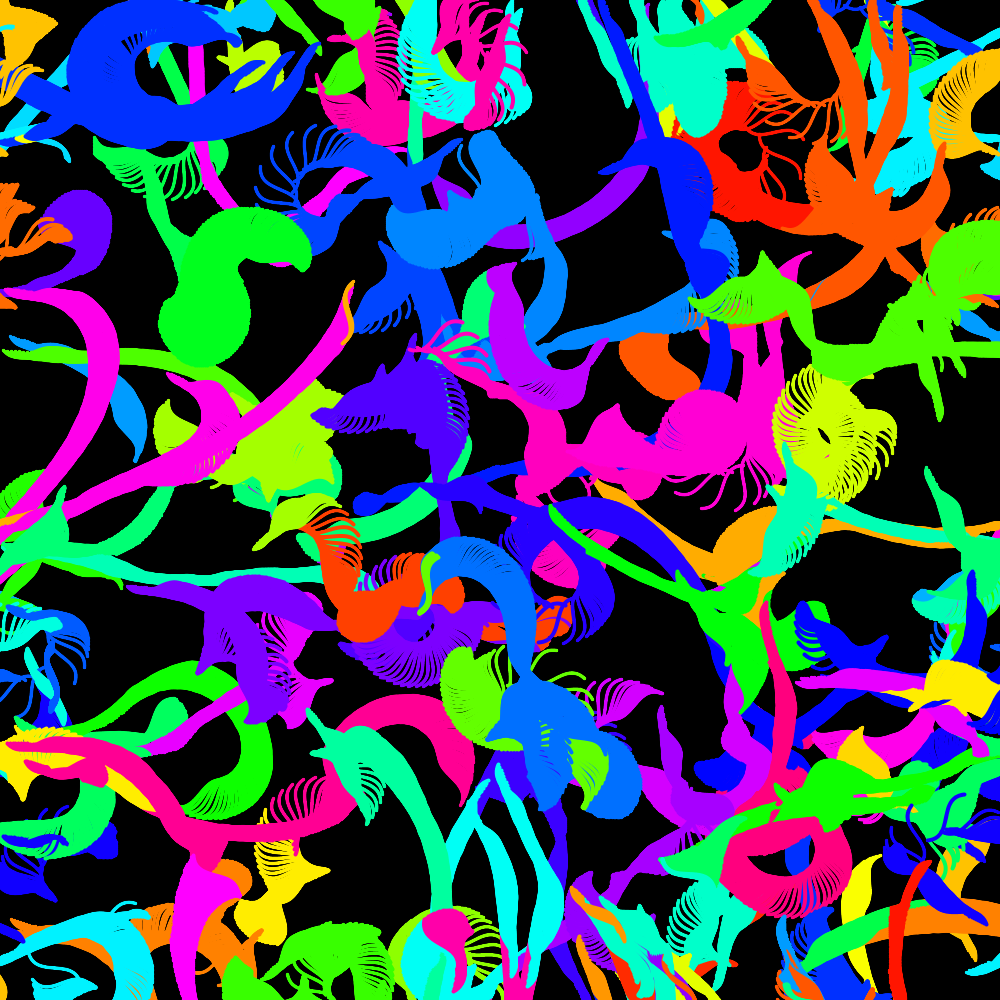
\includegraphics[width=0.5\linewidth]{img/schwarmKunst.png}
			\caption[SchwarmKunst]{Schwarm mit ausgeschaltetem Verlauf (eigene Darstellung)}
		\end{figure}
		
		
		\paragraph{Stärken und Schwächen}$~$\\
		Auch hier ist es faszinierend zu sehen, wie mit einem relativ einfachen Algorithmus ein Schwarmverhalten nachempfunden werden kann.\\
		Eine Schwäche liegt in der Laufzeit des Algorithmus. Wenn jeder Boid seine Position zu jedem anderen Boid prüfen muss, ergibt sich eine Laufzeit von O($ n^2 $). Der Quadtree bringt mehr Geschwindigkeit. Die Laufzeit kann auf O($ n \: log(n) $) verbessert werden, aber dadurch, dass dieser jedes Mal neu berechnet wird, wirkt sich dies erst richtig positiv bei großen Schwärmen aus.\\
		Der Algorithmus ist gut für die Einzelgenerierung geeignet. Man kann hier schon beeindruckende Bilder erhalten, erst recht, wenn man den Verlauf ausschaltet und die Punkte oder Kurven ihre Bahnen auch optisch ziehen.\\
		Auch bei der Kooperation kann man effektvolle Bilder erhalten. Hier kann man durch das ausgeschaltete Hindernis den Blick auf andere Bildelemente freihalten. Mit ausgeschaltetem Verlauf, ist der Schwarm eher für den Hintergrund geeignet. Auch sollte dann nur eine relativ kurze Iteration gewählt werden.\\
		
		\subsubsection{Evolutionärer Algorithmus}
		Auch für diesen Algorithmus liegt die Vorlage in der Biologie. Objekte sollen durch Evolution optimiert werden. Wie in der Natur gibt es eine Elterngeneration, die sich fortpflanzt und mit Hilfe der drei Schritte:
		\begin{itemize}
			\item Selection
			\item Crossover
			\item Mutation
		\end{itemize}
		die nächste Kindgeneration erschafft. Diese entwickelt sich im besten Fall näher auf ein Ziel zu. Danach wird diese Kindgeneration zur nächsten Elterngeneration usw.\\
		Der Algorithmus funktioniert so, dass zufällig generierte Objekte ein bestimmtes Ziel erreichen sollen, welches vorher definiert wurde. (Diese Ziele können z. B. sein: nimm eine bestimmte Farbe, eine bestimmte Richtung, eine bestimmte Form etc. an) Wie die Objekte dieses Ziel erreichen, wird aber nicht bestimmt. Es wird nur eine Fitnessfunktion geliefert, die die Objekte, die dieses Ziel zufällig erreicht haben, fitter machen. Durch die höhere Fitness der Individuen gelangt eine größere Anzahl von diesen Objekten, als von den weniger erfolgreichen Individuen (die Stärkeren überleben) in einen Paarungspool. Aus diesem Paarungspool werden dann zwei Elternteile gezogen (Selection), die durch Kreuzung (Crossover) neue Kinder für den Kinderpool erzeugen.
		Um die Vielfalt zu bewahren, werden zu einem geringen Prozentsatz auch wieder zufällige Objekte generiert (Mutation), die mit im neuen Kinderpool landen. Hieraus wird wieder der Elternpool und die Entwicklungs setzt sich fort bis der Algorithmus beendet und somit ein Ergebnis geliefert wird. (vgl. \cite{house2016autonomous})\\
		\paragraph{Beschreibung der Implementierung}$~$\\
		Die Implementierung erfolgte inspiriert von 'The nature of code' \cite{shiffman2012nature} wie oben beschrieben.
		Die Idee der Implementierung ist, dass eine Menge von Schnüren, die an einer bestimmten Stelle starten und eine zufällige Richtung, Farbe und Geschwindigkeit haben, sich auf ein Ziel ausrichten. Gleichzeitig behalten die Schnüre, die das Ziel erreichen ihre Farbe, so dass sich nach mehreren Generationen die Farben der Schnüre, die das Ziel erreichen, angleichen, bzw. im besten Fall übereinstimmen.\\
		Der Benutzer kann keinen Einfluss auf diese Evolution nehmen, sondern der Algorithmus arbeitet autonom. Die Anzahl der Schnüre und deren Startposition ist parametrisiert. Außerdem kann die Lebenszeit der Schnüre vom Benutzer eingestellt werden. Dies ist die Zeit, die den Schnüren bleibt, um ihr Ziel zu erreichen. Ist diese z. B. zu kurz, können sie zwar ihr Ziel nie erreichen, trotzdem wird die Ausrichtung aber nach einer gewissen Zeit in die Richtung des Ziel zeigen, da die Distanz des Schnurendes zum Ziel als Fitnesswert in die Berechnung einfließt. Durch die Evolution wird also auch hier den Schnüren, die sich auf das Ziel ausrichten der Vorzug gegeben.\\
		Inspiriert von ,,Autonomous Evolution of Digital Art Using Genetic Algorithms'' \cite{house2016autonomous} wurde noch eine Zielscheibe implementiert. Für die Viertelkreise etc. wurde ,,Processing - A Programming Handbook for Visual Designers and Artists'' \cite{reas2007processing} zu Hilfe genommen.\\ Hier hat der Benutzer nun die Möglichkeit zu wählen, wie viele Schnüre das Ziel treffen müssen, bevor sich die anfangs bunte Zielscheibe in eine einfarbige Scheibe verwandelt. Diese Verwandlung geschieht nach und nach, je nachdem wie viele Schnüre das Ziel schon getroffen haben, dabei färbt sich die Scheibe von innen nach außen gegen den Uhrzeigersinn einfarbig.\\
		Die Schnüre bilden sich aus Punkten, die sich auf dem Bildschirm bewegen. Dabei hat jede Schnur eine eigene DNA, die aus einer Farbe und einem  Vektor besteht, der dem Punkt eine Position, eine Richtung und eine Beschleunigung gibt.  Nachdem die Lebensspanne der Schnüre abgelaufen ist, wird die Fitness der Schnüre errechnet. Diese Funktion liefert die Distanz der Schnurenden zum Ziel. Um die Entwicklung noch zu beschleunigen, werden Schnüre, die eine Distanz unter 15 zum Ziel haben noch extra belohnt. Wie oben beschrieben landen Schnüre mit größerer Fitness in größerer Anzahl im nächsten Pool. Aus diesem Pool werden dann zufällig zwei Elternteile gezogen. Die Elternteile werden aber in diesem Algorithmus nicht gekreuzt, sondern es wird nur wiederum zufällig ein Elternteil als neues Kind gewählt. Diese Entwicklung wird so lange fortgesetzt, bis der Benutzer das Bild stoppt.\\
		Die Kooperation mit anderen Generatoren erfolgt auch hier mit den pseudozufälligen Variablen, die die Farbe und den Vektor initialisieren. Auch kann der Standort des Ziels von anderen Generatoren beeinflusst werden, wenn diese ein Interface benutzen, in dem sie diesen Punkt berechnen.\\
		Der Algorithmus gibt seinerseits den Standort der Schnüre als Kooperationspunkt weiter.\\
		
		\paragraph{Beispiele}$~$\\
		Unten kann man sehen, wie sich die Evolution unter den eingestellten Defaultwerten entwickelt. Nach 2100 Iterationen sieht man, dass mindestens 32 Schnüre die Zielscheibe getroffen haben und sich die Richtung der Schnüre eindeutig zum Ziel neigt. Die Farben haben sich vorrangig den lila Tönen angeglichen.\\
		Bildgenerierung links:,,Menübar/Beispiele/SHopf/Evolution/EvoDefault''\\
		Bildgenerierung rechts:,,Menübar/Beispiele/SHopf/Evolution/EvoDefaultEnd''\\
		\begin{figure}[H]
			\begin{minipage}[t]{0.45\linewidth} 
				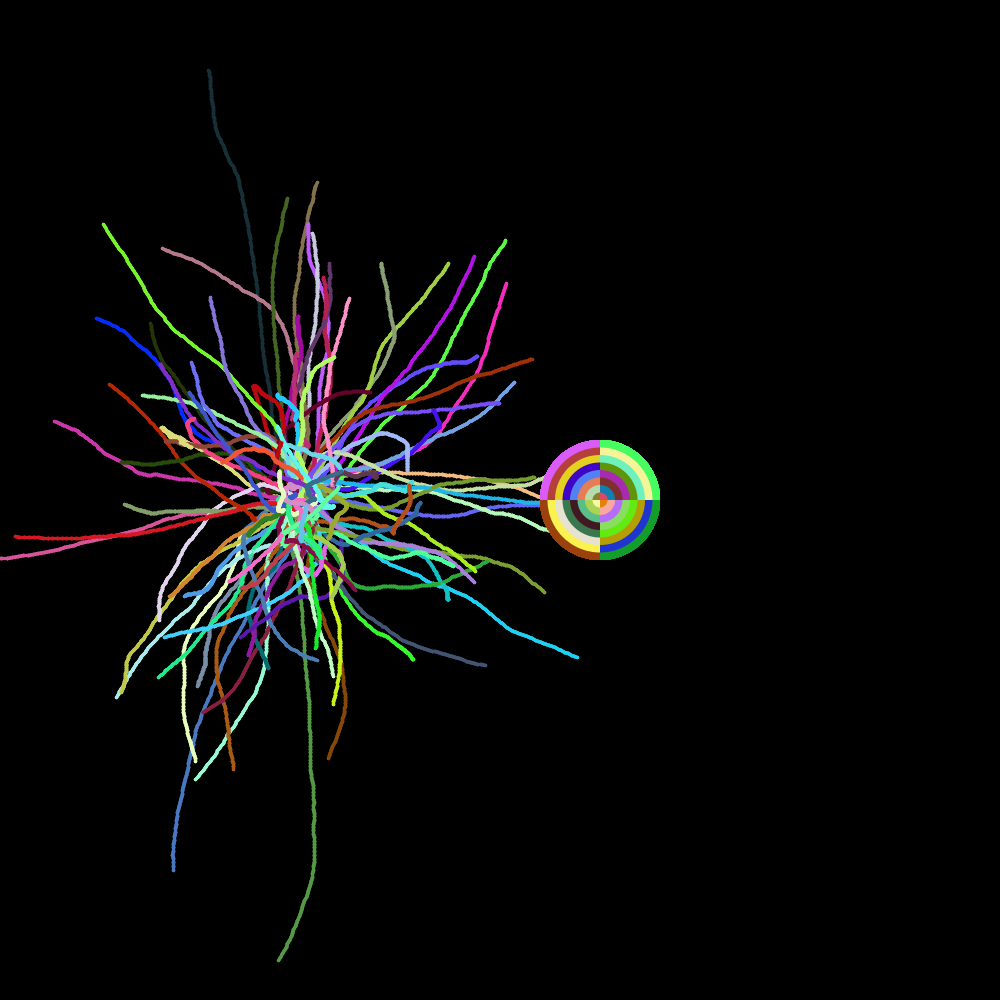
\includegraphics[width=\linewidth]{img/evoDefault.png}
				\caption[EvoDefault]{Evolution mit Defaultwerten nach 150 Iterationen (eigene Darstellung)}
			\end{minipage}
		\hfill
			\begin{minipage}[t]{0.45\linewidth} 
				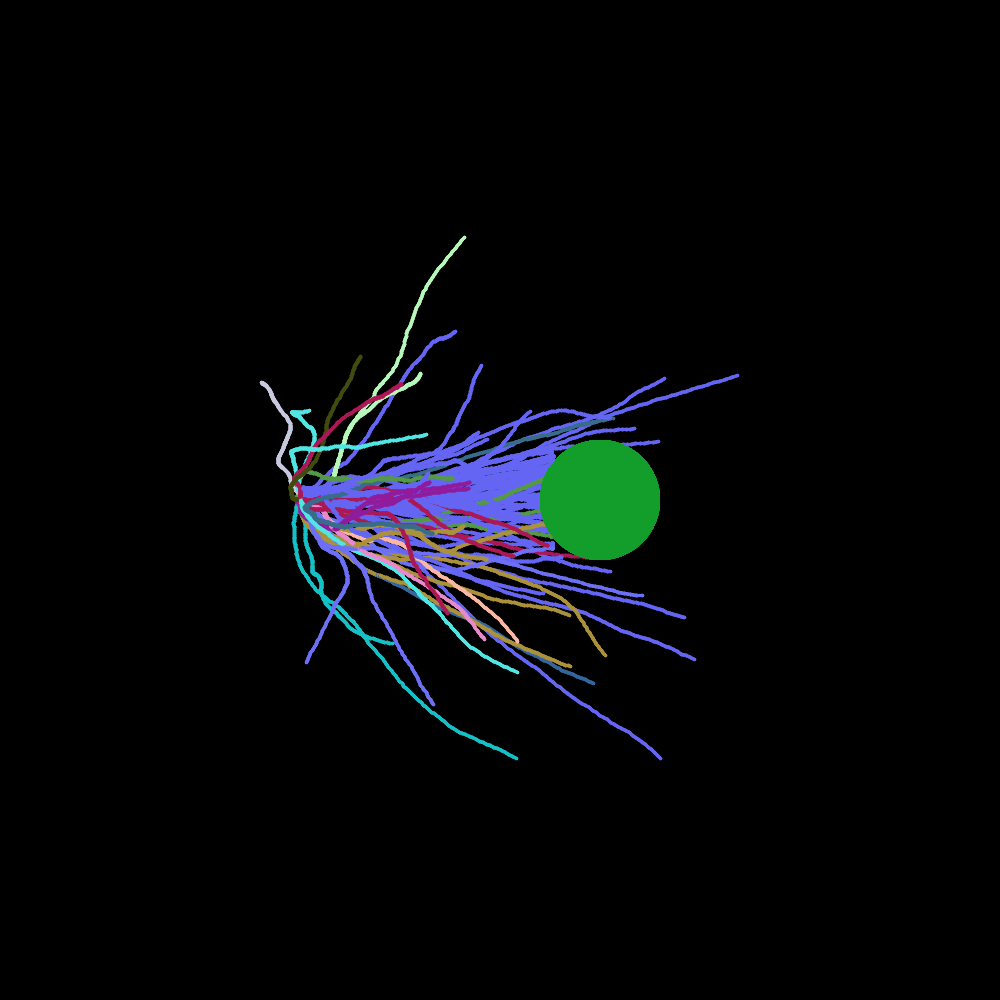
\includegraphics[width=\linewidth]{img/evoDefaultEnd.png}
				\caption[EvoDefaultEnd]{Evolution mit Defaultwerten nach 2100 Iterationen (eigene Darstellung)}
			\end{minipage}
		\end{figure} 
		\noindent Unten überströmen 300 Schnüre aus der linken oberen Ecke den Bildschirm, es sollten mindestens 75 Schnüre die Zielscheibe treffen. Nach 1800 Iterationen haben schon mindestens die Hälfte der angestrebten 75 Schnüre getroffen.\\
		Bildgenerierung:,,Menübar/Beispiele/SHopf/Evolution/EvoEcke''\\
		\begin{figure}[H]
			\centering
			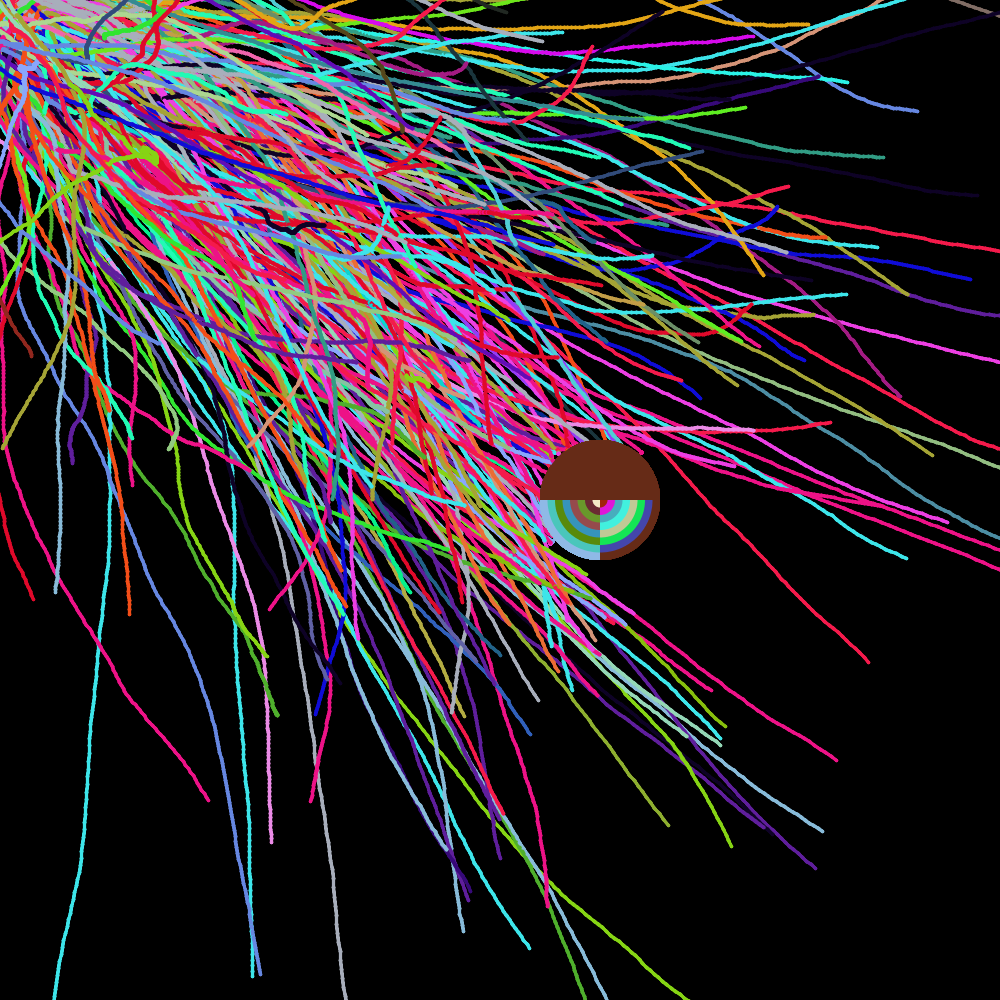
\includegraphics[width=0.5\linewidth]{img/evoEcke.png}
			\caption[EvoEcke]{Evolution mit 300 Schnüren nach 1800 Iterationen (eigene Darstellung)}
		\end{figure} 
		\noindent Unten nun eine Abbildung von nur 32 Schnüren, die alle die Zielscheibe treffen sollen. Hier muss man sehr viel Geduld aufbringen, falls man das vollständige Ergebnis sehen möchte, sofern dies überhaupt geschieht. Hier haben nach 6279 Iterationen noch nicht einmal die Hälfte der Schnüre getroffen. Die Farben haben sich aber schon angeglichen.\\
		Bildgenerierung:,,Menübar/Beispiele/SHopf/Evolution/EvoWenig''\\
		\begin{figure}[H]
			\centering
			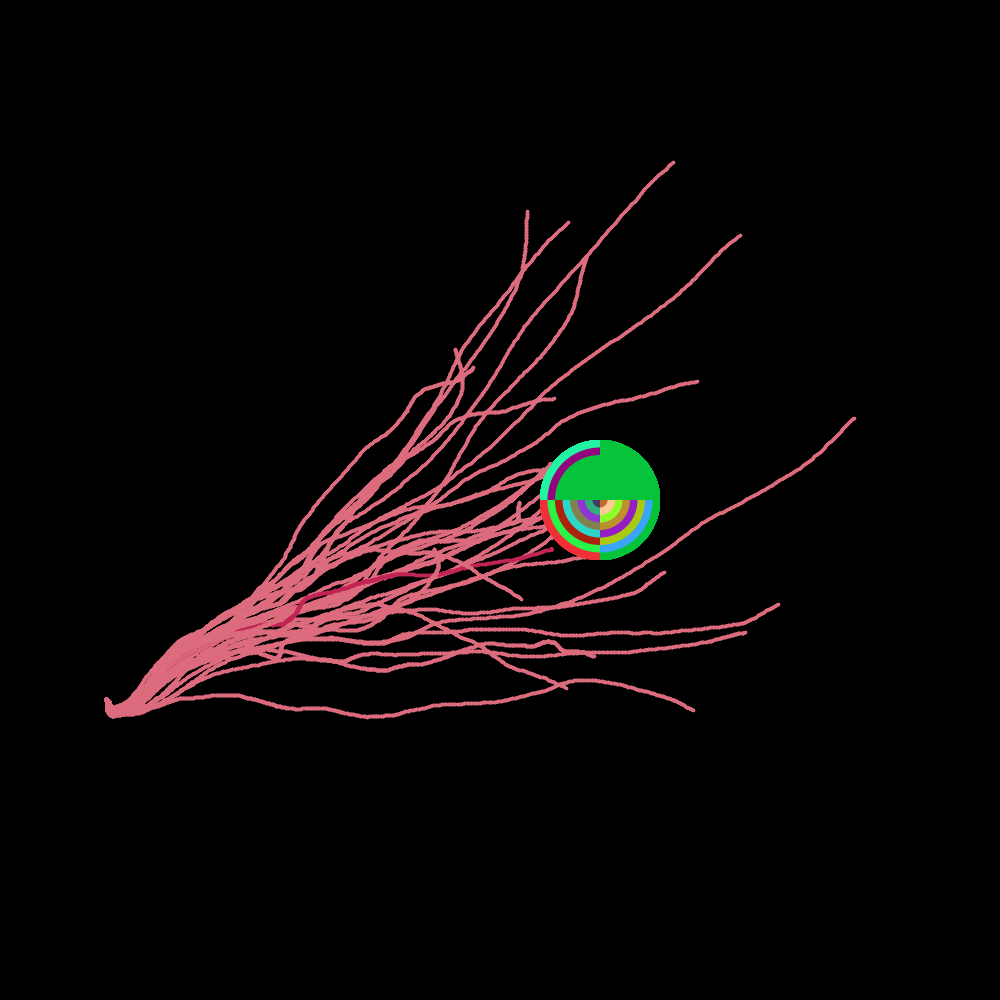
\includegraphics[width=0.5\linewidth]{img/evoWenig.png}
			\caption[EvoWenig]{Evolution mit 32 Schnüren nach 6279 Iterationen (eigene Darstellung)}
		\end{figure} 
				
		\paragraph{Stärken und Schwächen}$~$\\
		Die Stärken liegen hier vor allem in der selbstlernenden Art des Algorithmus. Wenn der Algorithmus mit echten Zufallszahlen läuft und man ein bestimmtes Ziel für ein Bild vor Augen hat, könnte man sich diesem auf immer neue Weise annähern und immer andersartige Kreationen erschaffen. Mit ein paar Modifizierungen könnte man hier auch den Benutzer mit einbinden, so dass er interaktiv an der Gestaltung von Bildern einwirken könnte.
		Die Schwächen liegen allerdings in der langen Laufzeit. Ein Bild ist nicht nach einer Lebensspanne der Objekte fertig, sondern braucht mehrere Generationen. Hier liegt es an dem Benutzer, wie viel Geduld er aufbringt.\\
		Der Algorithmus ist für die Kooperation und für die Einzelgenerierung geeignet, da er gut für sich allein wirkt, aber auch mit anderen Generatoren ein sehr schönes Ergebnis liefert. Hier können die anderen Generatoren dafür sorgen, dass das Ziel sich z. B. im L-System Baum befindet und die Schnüre auf diesen zusteuern usw.\\
		
	\subsubsection{Kooperation der eigenen Generatoren}
		Hier nun drei Beispiele, wie die eigenen Generatoren zusammenwirken können:\\
		Unten kooperieren ein L-System, ein Schwarm und ein weiteres L-System zusammen. Der rechte von den untersten Bäumen beeinflusst hier das Hindernis, dass der Schwarm meiden soll. Dies sieht man sehr schön an der freien Fläche rund um den Wipfel des Baumes.
		Außerdem werden von den Bäumen die Farbe und die Startinitialisierung der Boids beeinflusst. Der Schwarm seinerseits beeinflusst durch seine Einstellungen die Alphawerte der anderen Bäume und dass diese entartet sind.\\
		Bildgenerierung:,,Menübar/Beispiele/SHopf/Kooperation/Unterwasserwelt''\\
		\begin{figure}[H]
			\centering
			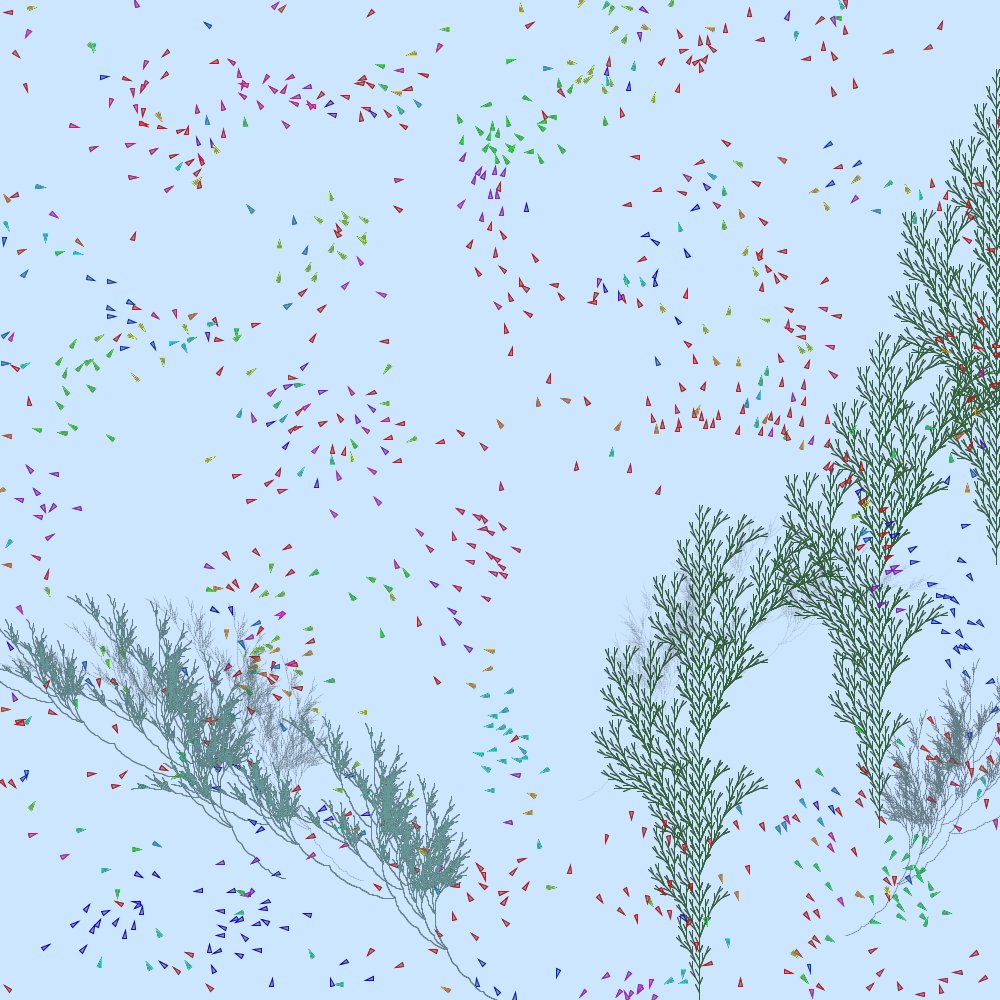
\includegraphics[width=\linewidth]{img/unterwasserwelt.png}
			\caption[Unterwasserwelt]{Kooperation L-System, Schwarm, L-System (eigene Darstellung)}
		\end{figure} 
		\noindent Unten kooperieren ein L-System, Evolution und ein weiteres L-System zusammen. Die oberen Bäume beeinflussen hier das Ziel der Evolutionsschnüre, welches sich wie man sieht in einem Baumwipfel befindet. Auch werden Farbe und Startinitialisierung der Schnüre von den Bäumen manipuliert. Die Evolution beeinflusst seinerseits den blauen Baum. Dieser wird dadurch in die andere Richtung gezeichnet.\\
		\begin{figure}[H]
			\centering
			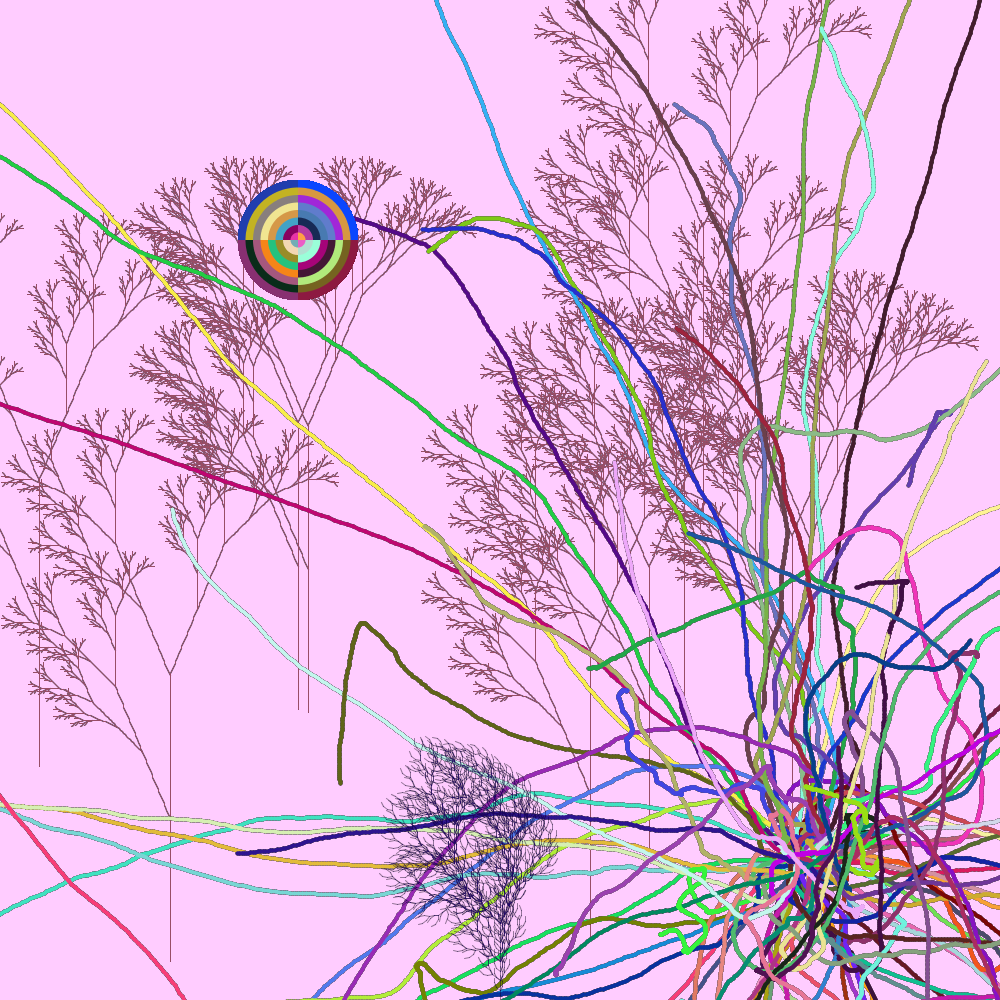
\includegraphics[width=\linewidth]{img/dschungel.png}
			\caption[Dschungel]{Kooperation L-System, Evolution, L-System (eigene Darstellung)}
		\end{figure} 
		\noindent Unten kooperieren ein Schwarm, Evolution und ein L-System zusammen. Der Schwarm zieht mit ausgeschaltetem Verlauf als Dreiecke seine Bahnen und beeinflusst das Ziel der Evolution. Die Startposition der Schnüre lenken ihrerseits die Ausrichtung der Bäume. Auch die Farben und Startinitialisierungen der Schnüre und die Größe der Bäume werden durch die Parameter der vorherigen Generatoren manipuliert.\\
	 	\begin{figure}[H]
	 		\centering
	 		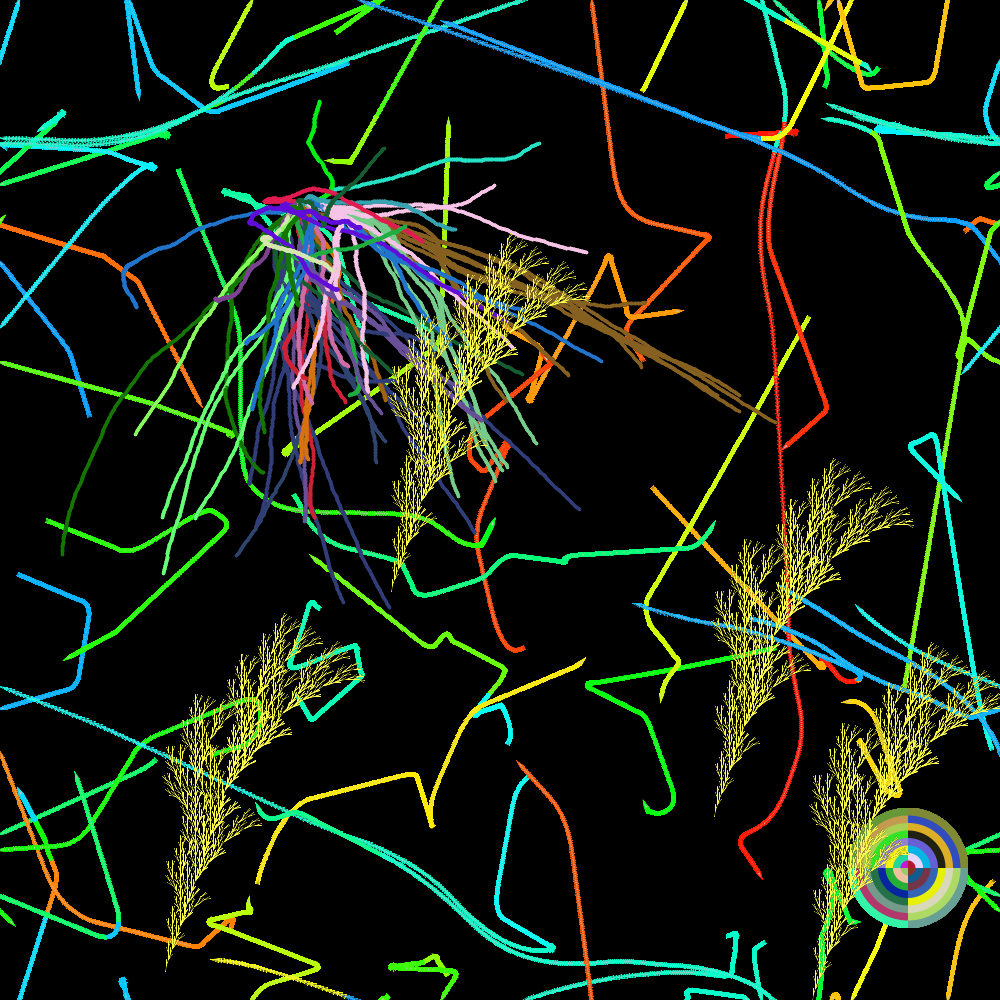
\includegraphics[width=\linewidth]{img/feuerwerk.png}
	 		\caption[Feuerwerk]{Kooperation Schwarm, Evolution, L-System (eigene Darstellung)}
	 	\end{figure} 
\end{document}